\documentclass{beamer}
\graphicspath{{./images/}}
\renewcommand\L{\mathcal{ L}}
\renewcommand{\epsilon}{\varepsilon}
\renewcommand{\div}[1]{\operatorname{div}\left( #1 \right)}
\usepackage{multimedia}
\usetheme{Warsaw}
\usecolortheme{beaver}
\title[Numerical homogenization]{Numerical Homogenization in Fenics}
%\subtitle{An exploration}
\author[O. Richardson \and I. Stefansson] % (optional, for multiple authors)
{Omar Richardson \and Ivar Stefansson}
\institute % (optional)
{
    Karlstad University, Sweden \and University of Bergen, Norway
}
\date[]{Nordic Computational Course, 2017}
\subject{Numerical Homogenization 1}

\begin{document}
  \frame{\titlepage}
\begin{frame}{Homogenisation}
    \begin{columns}
        \begin{column}[c]{.5\textwidth}
            Simulation of flow through nonhomogeneous media
            \begin{itemize}
              \item Conduction through composite materials
              \item Ground water flow
              \item Corrosion of concrete
            \end{itemize}
        \end{column}
        \begin{column}[c]{.5\textwidth}
            .
        \end{column}
    \end{columns}
\end{frame}

\begin{frame}[c]{Project aim}
    \begin{itemize}
        \item Implement automated upscaled solution solving in Fenics
        \item Obtain convergence rates w.r.t. mesh size and microstructure size
        \item Experiment with different solvers and preconditioners
    \end{itemize}
\end{frame}

\begin{frame}[t]{Model}
    Let $\varepsilon>0$. Find $u_\varepsilon(x)$ satisfying
    \begin{equation}
        \begin{split}
            -\div{A_\varepsilon(x)\nabla u_\varepsilon(x))} &= f(x) \mbox{ for } x \in \Omega,\\
            u_\varepsilon(x) &= 0 \mbox{ for } x \in \partial\Omega.
        \end{split}
        \label{eq:model}
    \end{equation}
     $A_\varepsilon(x)$ periodic with period $\varepsilon$.
     \begin{columns}
         \begin{column}[c]{.5\textwidth}
             \emph{i.e.}
             \[A_\varepsilon(x)= \frac{1}{2+\cos \left( \frac{2\pi x}{\epsilon} \right)}\]
         \end{column}
         \begin{column}[c]{.5\textwidth}
             \begin{figure}[th]
                \centering
                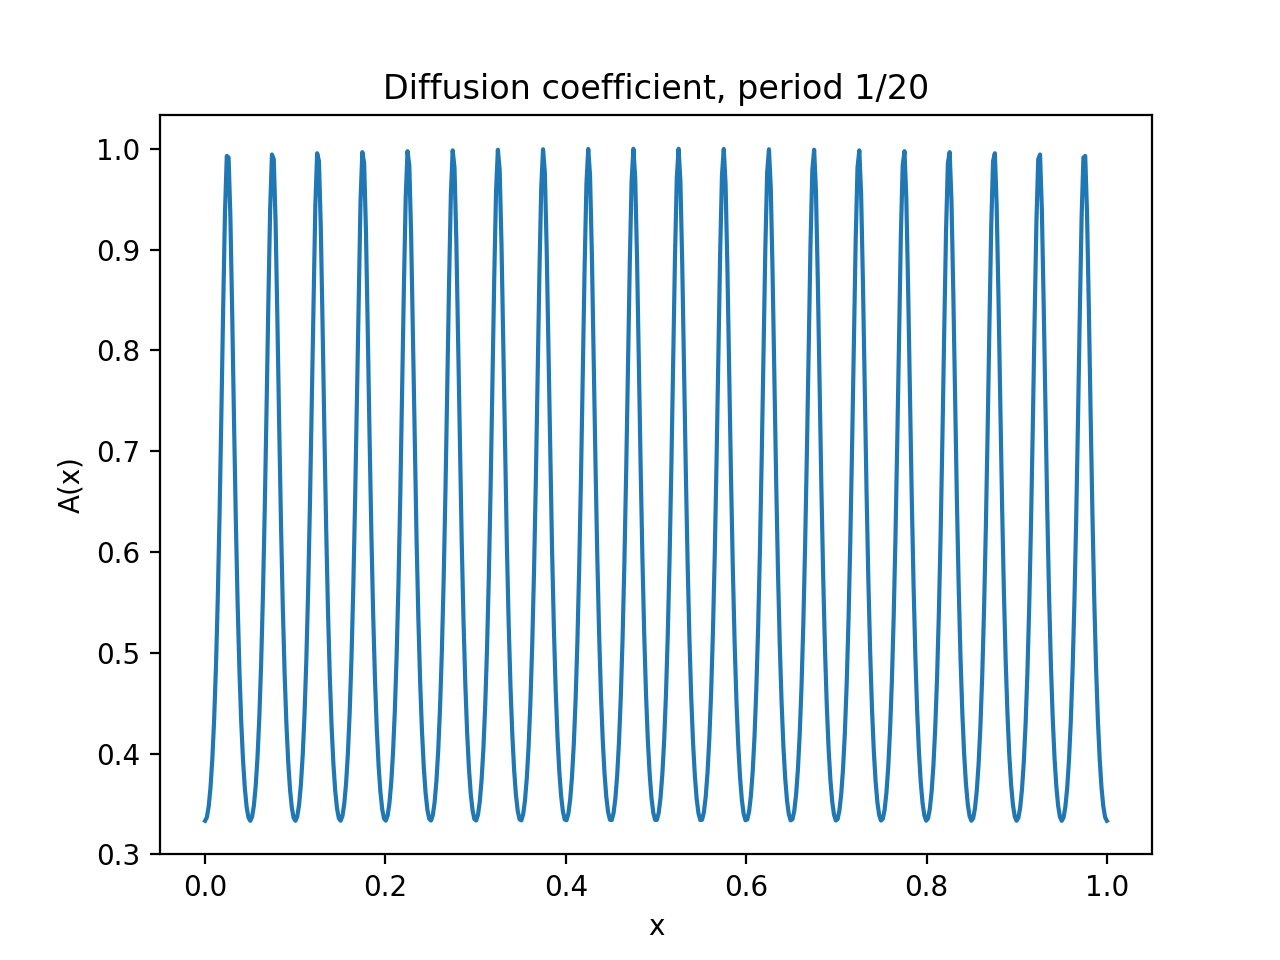
\includegraphics[width=0.9\linewidth]{a_eps.png}
                \caption{Plot of $A_\epsilon$ for $\epsilon=0.05$.}
                \label{fig:one_dim_exact}
            \end{figure}
         \end{column}
     \end{columns}

\end{frame}

\begin{frame}[t]{Upscaling}
    Two-scale separation: \begin{itemize}
        \item Macroscopic $x \in \Omega$, microscopic $y \in Y$.
        \[u_\varepsilon(x) = u(x,x/\varepsilon) = u(x,y)\]
        \item Ansatz: power expansion:
        \begin{equation*}
            u_\varepsilon(x,y) = \sum_i \varepsilon^i u_i(x,y)
            \label{eq:pow_exp}
        \end{equation*}
        %\item $\nabla u_i(x) = \varepsilon^{-1}\nabla_yu_i + \nabla_xu_i(x,y)$
    \end{itemize}
    then \emph{homogenized} solution $\lim_{\varepsilon\to 0} u_\varepsilon$ is obtained by solving for $u_0$.
\end{frame}

% \begin{frame}[c]{Weak Form}
%     Find $u \in H^1_0(\Omega)$ s.t.
%     \begin{equation}
%         \int_\Omega A_\epsilon\nabla u\nabla\phi dx= \int_\Omega f\phi dx
%         \label{eq:weak_form}
%     \end{equation}
%     for all $\phi \in H^1_0(\Omega)$.
% \end{frame}

\begin{frame}[t]{Exact solution}
  Synthetic version of Eq. \eqref{eq:model}:
  \begin{equation}
    \left( \frac{u'(x)}{2+\cos \left( \frac{2\pi x}{\epsilon} \right)} \right)' = 1
    \label{eq:one_dim}
  \end{equation}

  Allows for exact solution:
  \begin{equation}
    u(x) = \left( \frac{1}{2} - x \right) \left(2x + \frac{\epsilon}{2\pi}\sin\left(\frac{2\pi x}{\epsilon}\right) \right) + \frac{\epsilon^{2}}{(2\pi)^{2}}\left( 1 - \cos \left( \frac{2 \pi x}{\epsilon} \right) \right) + x^{2}
   \label{eq:one_dim_sol}
 \end{equation}
 \begin{figure}[th]
    \centering
    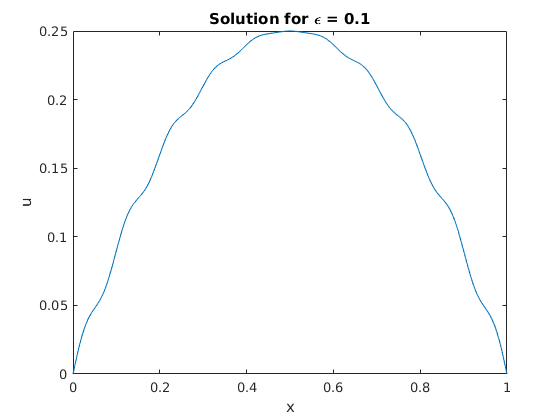
\includegraphics[width=0.35\linewidth]{one_dim_exact.png}
    \caption{Plot of the exact solution to \eqref{eq:one_dim} for $\epsilon=0.1 $.}
    \label{fig:one_dim_exact}
\end{figure}
\end{frame}

\begin{frame}[t]{Standard approximation}
\begin{columns}
    \begin{column}[c]{.5\textwidth}
      \begin{itemize}
      \item Now investigate the convergence for decreasing $\epsilon$ by comparing to the exact solution.
      \item Fourth order convergence provided $h$ resolves $\epsilon$
    \end{itemize}
  \end{column}
  \begin{column}[c]{.5\textwidth}

    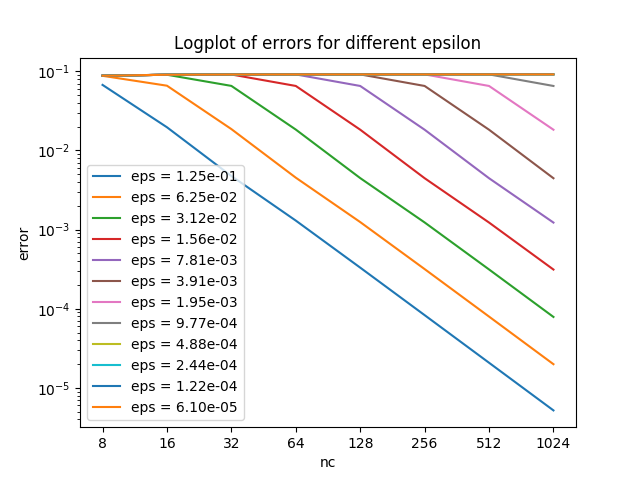
\includegraphics[width=0.85\linewidth]{one_dim_h_eps1.png}

    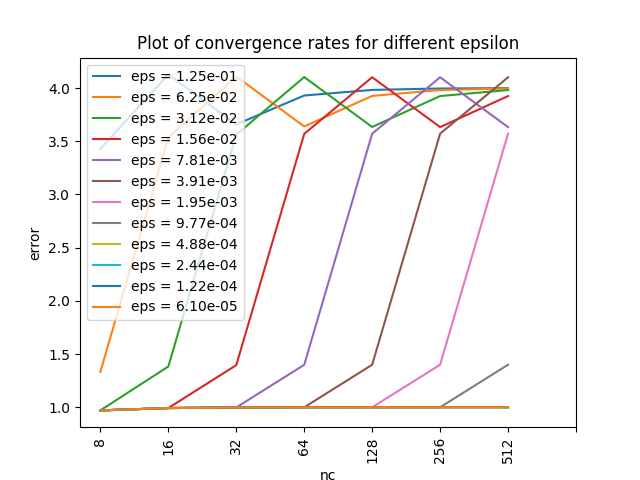
\includegraphics[width=0.85\linewidth]{one_dim_h_eps2.png}
 \end{column}
\end{columns}
\end{frame}


\begin{frame}[t]{2D upscaling}
\begin{columns}
    \begin{column}[t]{.5\textwidth}
      \begin{itemize}
          \item Two-dimensional example
           \[A_\epsilon(x) =  \left( 2+\cos\left(\frac{2\pi(x+2y)}{\epsilon}\right) \right)^{-1}\]
           Cell problem: for each unit vector $e_i$, find $w_i$ satisfying
           \[-\div{A(y)e_i} + \nabla_y w_i(y)) = 0\]
           \item Compute homogenized diffusion matrix $A^*_{ij}$ by
           \[A^*_{ij} = \int_Y(e_j + \nabla_y w_j)\cdot(e_i + \nabla_y w_i)dy\]
    \end{itemize}
  \end{column}
  \begin{column}[t]{.5\textwidth}
      \begin{figure}[th]
         \centering
         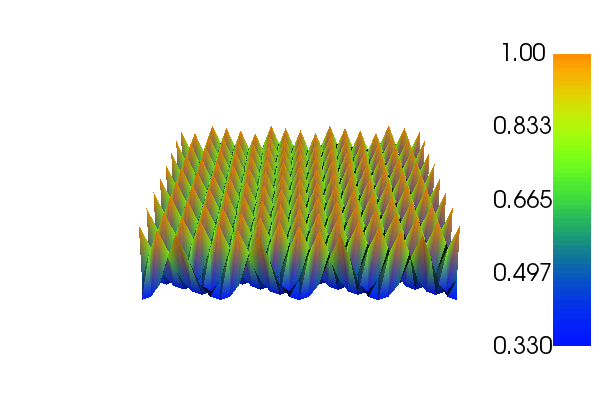
\includegraphics[width=0.85\linewidth]{two_dim_diff.png}
         \caption{Result of FeNiCS simulation of \eqref{eq:one_dim} for $\epsilon=0.1$ and $h = 1/80$}
         \label{fig:one_dim_approx}
     \end{figure}
 \end{column}
\end{columns}
\end{frame}


\begin{frame}[t]{2D upscaling: FeNiCS}
  \begin{columns}
    \begin{column}[c]{.6\textwidth}
      \begin{itemize}
        %\end{equation}
       \item High resolution for cell problem
       \item Remaining error:
      \begin{itemize}
        \item Model, $\epsilon > 0$
        \item Finite resolution in the solution of the global problem, $ h_{global} > 0$
        \item Convergence in both  $\epsilon$ and $h_{global}$.
       \end{itemize}
      \end{itemize}
    \end{column}
    \begin{column}[c]{.5\textwidth}
      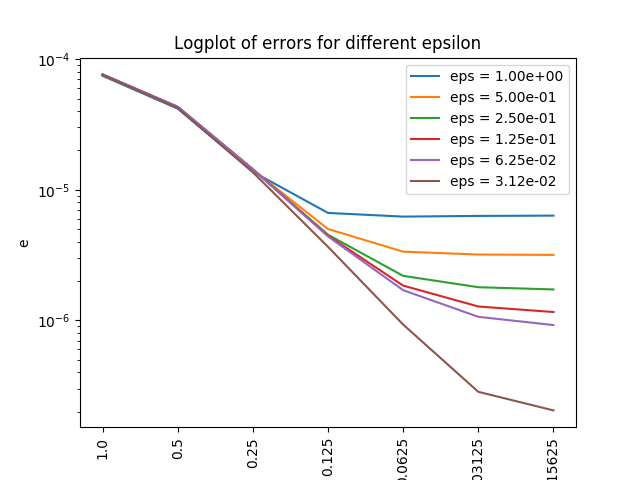
\includegraphics[width=0.9\linewidth]{2d_global_errors.png}      % 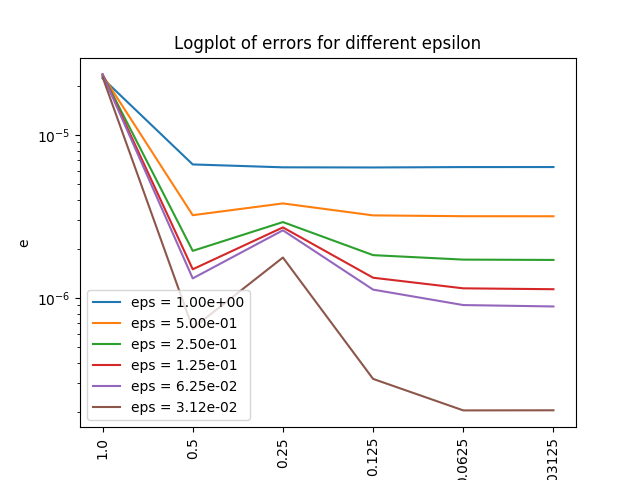
\includegraphics[width=0.65\linewidth]{2d_cell_errors.png}
    \end{column}
  \end{columns}
\end{frame}

\begin{frame}[t]{Solvers \& preconditioners}
  \begin{columns}
    \begin{column}[c]{.5\textwidth}
      \begin{itemize}
      \item Comparison of a selection of the solvers and preconditioners available in FEniCS.
      \item $~2.5\cdot10^{5}$ cells, both full and homogenized problem.
      \item Incomplete LU and Conjugate Gradient good for symmetric problems.
      \item GMRES expensive, convergence not granted for increased number of cells.
    \end{itemize}
  \end{column}
  \begin{column}[c]{.5\textwidth}

    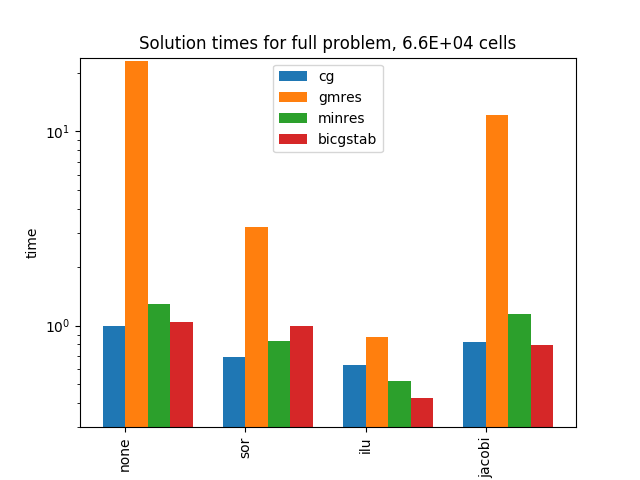
\includegraphics[width=0.9\linewidth]{SolverTimesFullh8.png}

    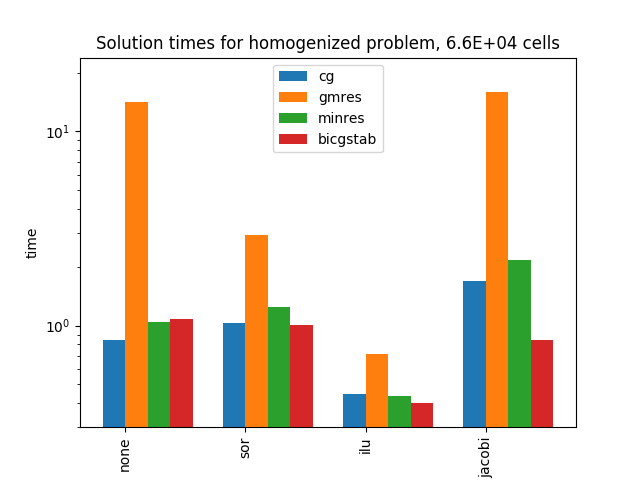
\includegraphics[width=0.9\linewidth]{SolverTimesHomoh8.png}

 \end{column}
\end{columns}
\end{frame}

\begin{frame}[t]{Application I}
  \begin{columns}
    \begin{column}[c]{.5\textwidth}
      \begin{itemize}
      \item Resolution of small $\epsilon$ unachievable due to complexity.
      \item Convergence in the  $\epsilon$ limit.
      \end{itemize}
      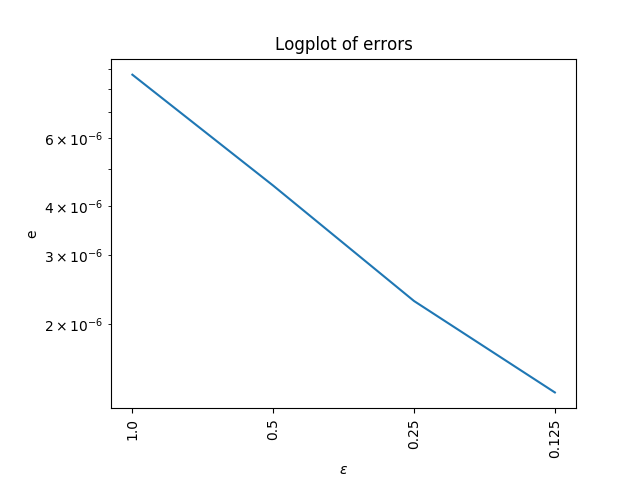
\includegraphics[width=0.65\linewidth]{carw_errors.png}
  \end{column}
  \begin{column}[c]{.5\textwidth}

    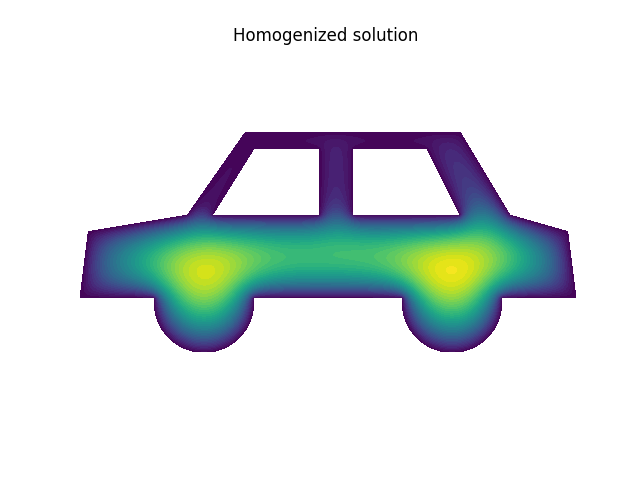
\includegraphics[width=0.65\linewidth]{carw_homogenized.png}

    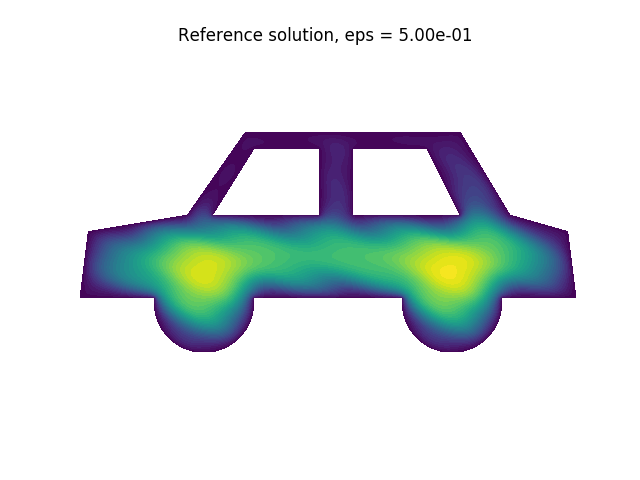
\includegraphics[width=0.65\linewidth]{carw_reference_eps_power_1.png}

    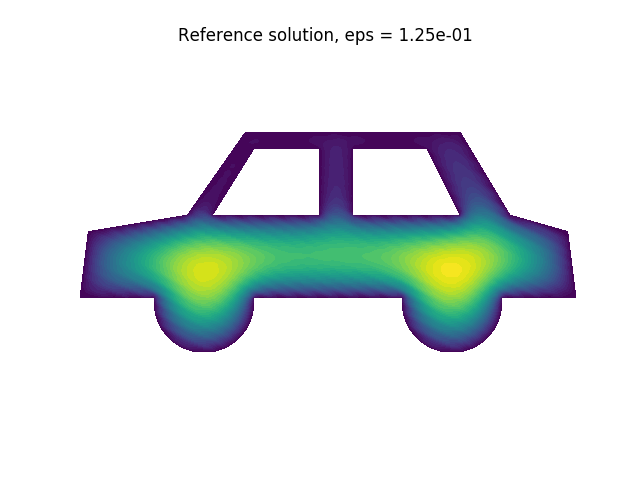
\includegraphics[width=0.65\linewidth]{carw_reference_eps_power_3.png}

 \end{column}
\end{columns}
\end{frame}

\begin{frame}[t]{Application II}
  \begin{columns}
    \begin{column}[c]{.5\textwidth}
      \begin{itemize}
      \item Three dimensions and time dependency add to computational cost.
      \item Homogenization usually only possibility, allows for simulations on a range of different applications.
    \end{itemize}
  \end{column}
  \begin{column}[c]{.5\textwidth}

 \end{column}
\end{columns}

\end{frame}
\end{document}
